\documentclass[conference]{IEEEtran}
\usepackage[T1]{fontenc}
\usepackage{amsmath,amssymb,graphicx,booktabs,array,tabularx}
\usepackage{cite}
\usepackage[hidelinks]{hyperref}
\usepackage{balance}
\newcolumntype{Y}{>{\raggedright\arraybackslash}X}
\newcolumntype{P}[1]{>{\raggedright\arraybackslash}p{#1}}
\newcommand{\MAE}{\operatorname{MAE}}
\newcommand{\LER}{\operatorname{LER}}
\newcommand{\CE}{\mathcal{L}_{\mathrm{CE}}}
\newcommand{\OLL}{\mathcal{L}_{\mathrm{OLL}}}
\newcommand{\MLL}{\mathcal{L}_{\mathrm{MLL}}}
\newcommand{\UnweightedAcc}{73.28}
\newcommand{\UnweightedMAE}{0.455}
\newcommand{\UnweightedFone}{0.454}
\newcommand{\BalancedFone}{0.538}
\newcommand{\MajorityAcc}{63.67}
\newcommand{\MajorityFone}{0.156}
\newcommand{\RemovedPct}{30.86}
\newcommand{\FiveStarPct}{63.72}
\newcommand{\TwoStarPct}{5.28}
\newcommand{\LongPct}{3.02}
\newcommand{\CPUName}{Apple M3 Pro}
\newcommand{\PythonVersion}{3.12.14}
\newcommand{\SklearnVersion}{1.9.1}
\newcommand{\VectorSeconds}{20.8}

\title{Product Review Rating Prediction:\\Progress Report on Data Preparation, Baselines,\\and Ordinal Learning Design}
\author{\IEEEauthorblockN{Efe Han Kele\c{s}, Mehmet Ege A\c{s}an, and Faris Aleem Ahmad}
\IEEEauthorblockA{CS 415 Project Progress Report\\November 16, 2026}}
\begin{document}
\maketitle

\begin{abstract}
Predicting a product review's one-to-five-star rating from its text requires both recognizing sentiment and accounting for the order of the labels. An error of one star is less severe than an error of four stars, although ordinary exact-match evaluation treats both as incorrect. This project investigates whether ordinal training objectives reduce rating distance and large errors while preserving macro-F1. This report reviews relevant literature, specifies a controlled TextCNN/DistilBERT comparison, and presents completed data preparation and preliminary experiments. A full audit of 568,454 Amazon Fine Foods reviews produced 393,001 usable, unique normalized texts after removing repeated and conflicting records. Product-disjoint training, validation, and test partitions were constructed and checked for exact text overlap. On 56,791 validation reviews, an unweighted TF--IDF linear baseline achieved \UnweightedAcc\% accuracy and \UnweightedMAE\ mean absolute error, averaged over three seeds. A class-balanced variant achieved \BalancedFone\ macro-F1, compared with \UnweightedFone\ for the unweighted model. These are preliminary baseline results; TextCNN, DistilBERT, and the ordinal-loss comparison remain future work. The reserved test set has not been used for prediction evaluation.
\end{abstract}
\begin{IEEEkeywords}
rating prediction, ordinal classification, sentiment analysis, TextCNN, DistilBERT
\end{IEEEkeywords}

\section{Problem and Motivation}
Online reviews contain detailed customer experiences, while star ratings compress those experiences into a small ordered scale. Our task is to infer a rating $y\in\{1,2,3,4,5\}$ using the review body $x$ alone. This can support feedback summarization or estimate the likely rating of an unrated written review. A prediction is an estimate of the expressed opinion, not a replacement for a customer's actual rating.

Several properties make the task difficult. Reviews may praise one aspect and criticize another; negation and long-distance context can reverse a sentiment cue. Different customers may attach different ratings to similar wording. The class frequencies are also unequal. A model that mostly predicts five stars can appear accurate while failing on dissatisfied customers and intermediate ratings. Finally, the labels are ordered: predicting five stars for a one-star review is more serious than predicting two stars.

The central research question is: \emph{Within a fixed model architecture, can an ordinal loss reduce mean absolute error and the frequency of errors of at least two stars without materially reducing macro-F1?} The original proposal specifies TextCNN and DistilBERT, each trained with cross-entropy (CE), ordinal log-loss (OLL), and multitask log loss (MLL). We retain this scope. The present progress consists of literature synthesis, an explicit evaluation protocol, a reproducible full-corpus audit, and measured linear baselines. We do not yet claim that the main research hypothesis has been confirmed.

\section{Related Studies and Their Implications}
\subsection{Rating Prediction and Strong Text Baselines}
Pang and Lee~\cite{pang2005}, in ACL, studied rating inference beyond binary positive/negative sentiment. Their metric-labeling formulation incorporates relationships among ratings and similarities among reviews. The important connection to our project is that rating prediction is not simply an unordered multiclass problem. Their method modifies classifier output through label relationships; our planned comparison instead changes the training objective while retaining a common five-output classifier.

Wang and Manning~\cite{wang2012}, in ACL, showed that feature choices and baseline variants can substantially change sentiment-classification performance. In particular, word bigrams and a combination of Naive Bayes features with SVMs were effective. This motivates measuring inexpensive lexical baselines before interpreting gains from neural models. Our TF--IDF logistic baseline follows this experimental principle; it is not a reproduction of their NB--SVM algorithm. Bigrams can represent short expressions such as ``not good,'' but cannot fully model sentence composition or distant context.

\subsection{Neural Text Representations}
Kim~\cite{kim2014}, in EMNLP, evaluated a convolutional sentence classifier using pretrained word vectors, convolutional filters, and max-over-time pooling. Static embeddings already performed strongly, while task-specific embedding updates could provide further gains. TextCNN offers a relatively inexpensive model of local word patterns and a useful reference architecture for this project. However, its pooling operation compresses sequence information, and a fixed embedding represents a word identically across contexts. These limitations motivate comparison with a contextual encoder rather than assuming a CNN is sufficient for every review.

Pennington et al.~\cite{glove2014}, in EMNLP, introduced GloVe, which learns word representations from global co-occurrence statistics. We plan to use its pretrained vectors as the frozen embedding layer in TextCNN. This keeps the proposal's static-embedding design and reduces the number of parameters that must be learned from the rating dataset. GloVe differs from the word-vector source used by Kim; our implementation will therefore be described as an adaptation of TextCNN, not an exact reproduction. Vocabulary coverage must still be measured on the training split.

Devlin et al.~\cite{bert2019}, in NAACL, introduced BERT's bidirectional pretraining and task-specific fine-tuning. Contextual representations provide a principled way to model interactions beyond local word windows. Sanh et al.~\cite{distil2019} compressed this approach through knowledge distillation in DistilBERT. Their reported speed and size benefits motivate a smaller Transformer under a course-project compute budget; they are not measurements on our hardware. DistilBERT is cited as an arXiv preprint, separately from the peer-reviewed conference and journal papers. Our experiment will test whether the effect of a loss function transfers from fixed-vector convolution to pretrained contextual representations.

Dang et al.~\cite{dang2021}, in \emph{Sensors}, combined BERT representations with CNN/LSTM classifiers and integrated sentiment information into a recommender system. Their five-level sentiment classification on Amazon Fine Food Reviews is especially relevant because it uses the same underlying review collection. Nevertheless, their recommendation component, feature pipeline, and evaluation setup differ from our text-only, product-disjoint task. Consequently, their scores cannot serve as directly comparable baselines for our experiment. Their study supports the dataset's applicability and the usefulness of learned representations, while our focus is a controlled comparison of training losses.

\subsection{Ordinal Methods and Evaluation}
Guti\'{e}rrez et al.~\cite{survey2016}, in \emph{IEEE Transactions on Knowledge and Data Engineering}, provide a taxonomy and experimental study of ordinal regression. Their discussion covers approaches that use ordering through model structure, decomposed binary problems, or thresholds. This establishes that there are several valid ways to incorporate order. Our choice of loss-based methods is primarily experimental: CE, OLL, and MLL can use the same five-class output layer, making architecture changes an avoidable confound.

Cao et al.~\cite{coral2020}, in \emph{Pattern Recognition Letters}, introduced CORAL to maintain rank consistency across binary ordinal subtasks. A five-level target can be represented through four ordered threshold decisions. This is an important alternative to a softmax classifier, but its output formulation differs from the proposed loss-only comparison. We retain CORAL as a possible extension after the main six configurations. Its published experiments concern age estimation; transfer of its benefits to review text requires evidence.

Chen et al.~\cite{chen2021}, in the Eval4NLP workshop, compared multiclass and ordinal formulations using the same underlying architecture. Their results illustrate that the preferred model can change when evaluation considers error magnitude rather than accuracy or F1 alone. This directly motivates reporting nominal and distance-sensitive metrics together. A reduction in mean error should not conceal poor recognition of minority classes, and improved macro-F1 should not conceal larger rating mistakes.

Castagnos et al.~\cite{oll2022}, in COLING, proposed OLL, which penalizes probability assigned to incorrect classes using their distance from the true class. Its distance exponent controls how strongly distant alternatives are penalized. The method is attractive here because it changes the objective without requiring a new encoder or label decomposition. The article evaluates multiple text benchmarks, but this does not establish that the method will satisfy our macro-F1 constraint under product-disjoint Fine Foods evaluation.

Kasa et al.~\cite{mll2024}, in Findings of ACL, compared explicit ordinal objectives and approaches that exploit label semantics. They introduced MLL as a weighted combination of CE and OLL to address the trade-off between nominal and ordinal performance. We adopt that published formulation and restrict the scope to the three specified losses. Their broader comparison motivates checking several metrics and treating the mixture weight as a validation hyperparameter. We do not assume that an ordinal objective guarantees either a unimodal predictive distribution or an empirical improvement on this dataset.

\subsection{Generalization and the Experimental Gap}
Blitzer et al.~\cite{blitzer2007}, in ACL, studied sentiment adaptation across Amazon product domains. Their binary classification setting differs from five-star prediction, but it shows why domain-dependent vocabulary matters. Product-disjoint splitting within Fine Foods addresses unseen products within a category; it does not establish generalization to a different category, platform, or time period. Cross-category evaluation remains optional, after the main experiment is complete.

Taken together, the literature motivates our representations, ordinal objectives, and evaluation measures. Our contribution is a reproducible comparison of existing methods under a common data protocol, not a new loss function. Table~\ref{tab:literature} summarizes the resulting design choices.

\begin{table*}[t]
\caption{How the reviewed literature informs the project. Published results are not treated as directly comparable project scores.}
\label{tab:literature}
\centering\footnotesize
\begin{tabularx}{\textwidth}{@{}P{0.22\textwidth}P{0.29\textwidth}Y@{}}
\toprule
Study and venue & Main methodological contribution & Consequence for this project\\
\midrule
Pang--Lee, ACL 2005 & Rating-scale relationships and metric labeling & Treat ratings as ordered labels; retain distance-sensitive evaluation.\\
Wang--Manning, ACL 2012 & Strong lexical models and word bigrams & Establish a measured lexical reference before neural comparisons.\\
Kim; Pennington et al., EMNLP 2014 & Convolutional classification; pretrained GloVe vectors & Use local-pattern convolution with frozen pretrained embeddings.\\
Devlin et al., NAACL 2019; Sanh et al., preprint & Contextual pretraining; model distillation & Compare a fine-tuned DistilBERT encoder with TextCNN.\\
Dang et al., Sensors 2021 & Hybrid sentiment/recommendation on Fine Foods & Supports domain relevance; differing protocols prevent score equivalence.\\
Guti\'{e}rrez et al., IEEE TKDE 2016; Cao et al., PRL 2020 & Ordinal taxonomy; rank-consistent thresholds & Recognize alternatives, but hold the output structure fixed in the main study.\\
Chen et al., Eval4NLP 2021 & Error-sensitive assessment of ordered labels & Jointly report accuracy, macro-F1, MAE, and large error rate.\\
Castagnos et al., COLING 2022; Kasa et al., Findings ACL 2024 & OLL; CE/OLL mixture and comparative analysis & Compare CE, OLL, and MLL with matched model and data settings.\\
Blitzer et al., ACL 2007 & Cross-domain sentiment adaptation & Separate within-category product generalization from optional domain transfer.\\
\bottomrule
\end{tabularx}
\end{table*}

\section{Activities: Theoretical Design and Justification}
\subsection{Input Definition and Data Protocol}
The model input is the review body. The star rating is the target; product IDs are used only to construct partitions. User IDs, helpfulness votes, summaries, and other metadata are excluded from the predictors. This makes the experiment a direct test of information in the review body and avoids incorporating metadata unavailable for an unrated review.

The implemented normalization decodes HTML entities, removes HTML tags, collapses repeated whitespace, and lowercases the text. It does not stem words or remove stopwords, so negation words remain available. Reviews with missing text, missing product IDs, or ratings outside $1$--$5$ are rejected. We group records by normalized body text, remove all records in a group if its labels disagree, and retain the first source record in each remaining repeated-text group. This is a deterministic corpus-curation rule, fixed before model fitting. It defines a deduplicated task and is not a method for resolving the ambiguity of conflicting reviews.

We then assign each retained product ID to train, validation, or test using a salted SHA-256 hash with probability intervals $[0,0.70)$, $[0.70,0.85)$, and $[0.85,1)$. This assigns all retained reviews of a product to the same partition without using the rating. Review-level proportions need not be exactly 70/15/15 because products have unequal numbers of reviews. The salt and row-level assignment are saved. Vocabulary and inverse document frequencies are fitted on training text only. Test labels are used for fixed curation and descriptive counts, but no test predictions or model-selection scores are computed.

\subsection{Architecture Decisions}
\textbf{TextCNN (specified; not yet trained).} The starting configuration uses 100-dimensional frozen GloVe embeddings, convolution widths 3, 4, and 5, 100 filters per width, ReLU, max-over-time pooling, dropout 0.5, and a five-output linear layer. These are provisional implementation settings, not selected experimental winners. The training vocabulary will be capped at 50,000 tokens, with explicit padding and unknown-token handling. A 256-token input limit is the initial memory-budget choice; truncation and embedding coverage will be measured before freezing it.

\textbf{DistilBERT (specified; not yet trained).} We plan to fine-tune \texttt{distilbert-base-uncased} with its tokenizer and a five-output classification head, updating both encoder and head. The starting maximum length is 256 subword tokens and the batch size is 16, subject to a memory pilot. Word counts are not interchangeable with Transformer token counts. Any revision to sequence length or batch size will be fixed across all losses within this architecture before the comparative runs.

These architectures provide complementary inductive biases: local pattern extraction with frozen vectors and contextual representation learning through fine-tuning. Their absolute scores also depend on pretraining and capacity. We therefore interpret a loss effect primarily \emph{within} an architecture, rather than attributing all cross-architecture differences to ordinality.

\subsection{Loss Functions and Decision Rule}
Let $p_k=\operatorname{softmax}(z)_k$ be the predicted probability of star class $k$. We use integer star distance $d(y,k)=|y-k|$. This treats successive star steps as equally costly, an explicit operational assumption rather than a claim about equal psychological distances.
\begin{align}
\CE(p,y)&=-\log p_y,\label{eq:ce}\\
\OLL(p,y)&=-\sum_{k\ne y}|y-k|^{\alpha}\log(1-p_k),\label{eq:oll}\\
\MLL(p,y)&=\lambda\CE(p,y)+(1-\lambda)\OLL(p,y).
\label{eq:mll}
\end{align}
Equation~\eqref{eq:oll} follows Castagnos et al.~\cite{oll2022}; Eq.~\eqref{eq:mll} follows Kasa et al.~\cite{mll2024}. We retain unnormalized distances, record $\alpha$ and $\lambda$, and do not silently divide the ordinal term by the number of classes. Changing its scale changes the effective mixture. Stable log-probability operations will be used in the trainable implementation, with numerical checks near the simplex boundaries.

CE rewards the correct class probability, whereas OLL also distinguishes where incorrect probability is placed. MLL preserves direct supervision of the correct class while applying an ordinal penalty. A computed illustration in Table~\ref{tab:loss} holds $p_y$ fixed and moves mass from a nearby class to a distant one. This verifies the intended numerical behavior; it is not evidence of trained-model accuracy.

\begin{table}[t]
\caption{Computed loss illustration, not a trained experiment. True rating is 1, $\alpha=1$, and $\lambda=0.5$.}
\label{tab:loss}
\centering\footnotesize
\begin{tabular}{@{}lrrr@{}}
\toprule
Probability mass pattern & CE & OLL & MLL\\\midrule
Near-error vector & 2.303 & 1.904 & 2.103\\
Far-error vector & 2.303 & 6.652 & 4.477\\
\bottomrule
\end{tabular}
\par\smallskip\parbox{\columnwidth}{\scriptsize Near: $(.10,.80,.04,.03,.03)$. Far: $(.10,.03,.03,.04,.80)$. Entries follow star order 1--5.}
\end{table}


All principal comparisons will use $\hat y=\arg\max_k p_k$. The same rule prevents a change in decoding from being mistaken for a change in training loss. Posterior-median decoding, which is relevant to absolute-error minimization when probabilities are reliable, can be a separately labeled ablation. It will not replace argmax in selected rows of the main comparison.

\subsection{Controlled Comparison and Success Criteria}
The core design contains $2\times3=6$ architecture/loss settings. Each final setting will be run with seeds 17, 29, and 43 on the same data assignment. Within an architecture, paired runs will use the same initial encoder/head state and data order where technically possible. We will fix preprocessing, batch size, optimizer family, maximum epochs, and checkpoint-selection rules within each architecture, then allow a comparable validation-search budget per loss. Loss magnitude affects optimization, so forcing a single learning rate without a pilot could itself introduce an unfair comparison.

The proposed search has six candidate configurations per loss per architecture. CE varies learning rate and weight decay; OLL varies learning rate and $\alpha\in\{1,2\}$; MLL initially fixes $\alpha=1$ and varies learning rate and $\lambda\in\{0.25,0.5,0.75\}$. The exact learning-rate values will be frozen after a training-only stability pilot. This restricted MLL search does not explore all combinations of exponent and mixture weight. Search runs use seed 17; the chosen configuration is then evaluated across all three seeds. Checkpoints are selected by validation MAE, with higher macro-F1 breaking ties, under a common maximum-epoch and patience policy within each architecture.

For $N$ predictions, we compute
\begin{align}
\MAE &=\frac{1}{N}\sum_{i=1}^{N}|\hat y_i-y_i|,\\
\LER &=\frac{1}{N}\sum_{i=1}^{N}\mathbf{1}\{|\hat y_i-y_i|\ge2\}.
\end{align}
Accuracy measures exact matches and macro-F1 averages the five classwise F1 values with equal weight. LER is also one minus off-by-one accuracy. We will report all four metrics, per-class results, confusion matrices, and measured time on the same hardware.

The proposal's success criterion remains unchanged: relative to CE within an architecture, at least one ordinal method must reduce MAE by at least 3\% and LER by at least 5\%, while its macro-F1 decrease is no more than 0.01 on the 0--1 scale. These are joint requirements on the three-seed mean test results, not already achieved outcomes. When final evaluation is performed, paired product-level bootstrap intervals will complement seed standard deviations; reviews from the same product must not be treated as independent bootstrap units. Trying two ordinal losses across two architectures also requires caution when interpreting a single favorable configuration.

\begin{figure*}[t]
\centering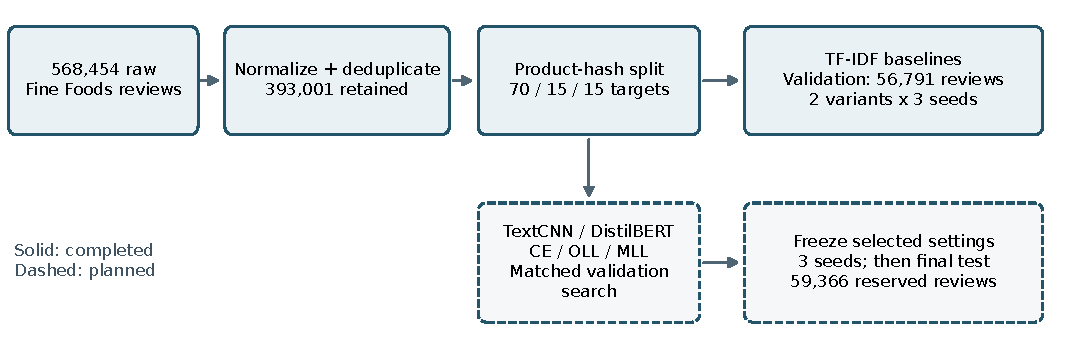
\includegraphics[width=0.97\textwidth]{figures/pipeline.pdf}
\caption{Current workflow and the planned main experiment. Solid boxes show completed processing and baseline evaluation. Dashed boxes show the neural comparison and final test evaluation that remain to be performed.}
\label{fig:pipeline}
\end{figure*}

\section{Activities: Experiments and Results}
\subsection{Completed Work and Evidence}
The original proposal selected the task, candidate datasets, architectures, and success thresholds. Earlier local checks inspected non-random prefixes of several candidate datasets; those checks verified basic structure but were not representative performance experiments. The present work extends this to the complete primary corpus, reproducible partitioning, and six trained linear-baseline runs. Table~\ref{tab:status} explicitly separates completed work from planned work.

\begin{table}[t]
\caption{Progress as of November 16, 2026.}
\label{tab:status}\centering\footnotesize
\begin{tabularx}{\columnwidth}{@{}Y P{0.24\columnwidth}@{}}
\toprule Activity & Status\\\midrule
Literature synthesis and method justification & Completed\\
Full Fine Foods audit and deterministic cleaning & Completed\\
Product-disjoint split and exact-overlap checks & Completed\\
TF--IDF baselines, two variants, three seeds each & Completed\\
Numerical CE/OLL/MLL illustration & Completed\\
TextCNN and DistilBERT architecture specification & Designed\\
Neural training and comparative loss experiments & Pending\\
Final test evaluation and optional domain transfer & Pending\\
\bottomrule
\end{tabularx}
\end{table}

\subsection{Full-Corpus Audit}
The downloaded SNAP archive~\cite{finefoods} contains 568,454 records and 74,258 distinct product IDs, matching the published counts. Its checksum and source URL are saved in the experiment artifacts. All records passed the implemented checks for nonempty normalized text, valid ratings, and product IDs. This is not a certification of language, authenticity, or semantic agreement between text and rating.

The audit found 119 normalized-text groups with inconsistent ratings, containing 428 records. Removing these groups and then 175,025 redundant same-label records leaves 393,001 reviews and 67,485 retained products. The 175,453 removed rows represent \RemovedPct\% of the raw collection. Global exact-text deduplication prevents identical retained texts from appearing across partitions. However, keeping only the first occurrence changes the product and review distribution; this is a deliberate definition of the cleaned evaluation corpus. Near duplicates, spelling variants, and product aliases remain potential leakage channels.

\begin{table}[t]
\caption{Measured data-curation counts on the full archive.}
\label{tab:audit}
\centering\footnotesize
\begin{tabular}{@{}lr@{}}
\toprule
Item & Count\\\midrule
Raw reviews & 568,454\\
Raw products & 74,258\\
Invalid or missing-field rows & 0\\
Conflicting normalized-text groups & 119\\
Rows in conflicting groups removed & 428\\
Same-label duplicate rows removed & 175,025\\
Retained reviews & 393,001\\
Retained products & 67,485\\
\bottomrule
\end{tabular}

\end{table}

\begin{table}[t]
\caption{Retained review counts by star rating and partition. Test data are reserved for final prediction evaluation.}
\label{tab:splits}
\centering\footnotesize
\begin{tabular}{@{}lrrr@{}}
\toprule
Stars & Train & Validation & Test\\\midrule
1 & 25,369 & 5,343 & 5,482\\
2 & 14,672 & 3,034 & 3,056\\
3 & 21,339 & 4,173 & 4,193\\
4 & 39,927 & 8,084 & 7,920\\
5 & 175,537 & 36,157 & 38,715\\
Total & 276,844 & 56,791 & 59,366\\
Products & 47,394 & 9,892 & 10,199\\
\bottomrule
\end{tabular}

\end{table}


Five-star reviews constitute \FiveStarPct\% of the cleaned corpus, while two-star reviews constitute \TwoStarPct\%. Figure~\ref{fig:data} shows that the training and validation distributions remain strongly skewed. This explains why accuracy alone would be misleading. The median normalized review length is 56 whitespace-delimited words; the 95th percentile is 213, and \LongPct\% exceed 256 words. These values justify measuring truncation explicitly rather than assuming that a 256-token neural input preserves all relevant content.

\begin{figure}[t]
\centering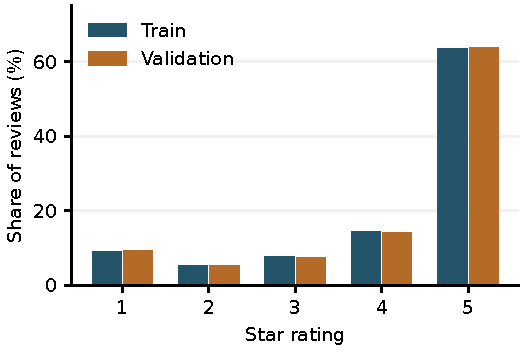
\includegraphics[width=\columnwidth]{figures/data_profile.pdf}
\caption{Measured class frequencies in the cleaned training and validation splits. Counts and preprocessing come from the full-corpus audit.}
\label{fig:data}
\end{figure}

The partitions contain 276,844 training, 56,791 validation, and 59,366 reserved test reviews. Assertions over every pair of splits verified zero shared retained product IDs and zero shared normalized-text hashes. This establishes the intended exact-overlap constraints, not general independence: users can still recur and semantically equivalent product variants may have different identifiers.

\subsection{Baseline Setup}
We evaluated a majority-class predictor and two lexical classifiers. The majority predictor chooses the most frequent training rating, which is five stars. Both learned variants use identical TF--IDF unigram and bigram features, a training-only vocabulary of at most 60,000 features, minimum document frequency 3, sublinear term frequency, and L2 normalization. The tokenizer retains word tokens of at least two characters. Thus negation words are retained, although punctuation and some contractions are simplified by tokenization. This feature policy is a baseline choice, not the final neural tokenization.

The classifier is scikit-learn's \texttt{SGDClassifier} with binary logistic loss in a one-versus-rest multiclass formulation, L2 penalty $10^{-5}$, at most 30 epochs, tolerance $10^{-4}$, and default optimal learning-rate schedule. It is \emph{not} the five-way softmax CE model specified for the neural comparison. The unweighted variant uses uniform sample importance. The balanced variant uses training-derived class weights $n/(5n_c)$ to increase the contribution of less frequent ratings. We do not equate class weighting with an ordinal loss.

Both variants were trained with seeds 17, 29, and 43. Hyperparameters were fixed for this preliminary experiment; no grid search selected the reported rows. We evaluate on validation only and use the same partition for every seed and variant. Training runs used one CPU thread on an \CPUName\ system, with Python \PythonVersion\ and scikit-learn \SklearnVersion. Feature construction and validation transformation together took \VectorSeconds\ seconds. The reported fit time excludes feature extraction and prediction; timing is a local measurement, not a benchmark of neural-model efficiency.

\subsection{Measured Validation Performance}
\begin{table*}[t]
\caption{Validation performance: mean $\pm$ sample standard deviation over seeds 17, 29, and 43. Accuracy and LER are percentages; macro-F1 uses the 0--1 scale; MAE is in stars. The deterministic majority baseline is evaluated once.}
\label{tab:baselines}
\centering\footnotesize
\begin{tabular}{@{}lccccc@{}}
\toprule
Model & Accuracy $\uparrow$ & Macro-F1 $\uparrow$ & MAE $\downarrow$ & LER $\downarrow$ & Fit time (s)\\\midrule
Majority & 63.67 & 0.1556 & 0.8259 & 22.10 & --\\
TF--IDF, unweighted & $73.28 \pm 0.02$ & $0.4538 \pm 0.0012$ & $0.4550 \pm 0.0009$ & $10.35 \pm 0.03$ & $8.75 \pm 0.72$\\
TF--IDF, balanced & $73.54 \pm 0.01$ & $0.5376 \pm 0.0004$ & $0.3956 \pm 0.0004$ & $7.75 \pm 0.03$ & $10.75 \pm 0.29$\\
\bottomrule
\end{tabular}

\end{table*}

Table~\ref{tab:baselines} reports means and sample standard deviations across the three optimization seeds. The majority predictor obtains \MajorityAcc\% accuracy while macro-F1 is only \MajorityFone. Its apparent accuracy mainly reflects label imbalance and gives a necessary lower reference for interpreting the learned models.

The unweighted lexical classifier improves accuracy to 73.28\%, macro-F1 to 0.4538, and MAE to 0.4550. The balanced variant reaches 73.54\% accuracy and 0.5376 macro-F1, with MAE 0.3956 and LER 7.75\%. Compared with the unweighted model, balancing reduces MAE by 13.05\% and LER by 25.10\% relative, while increasing macro-F1 by 0.0839. All four aggregate metrics improve in this pilot; the remaining trade-offs occur at the classwise precision/recall level. These gains concern class weighting in a linear model, so they do not satisfy or test the proposal's CE-versus-ordinal-loss success criterion. All six fits terminated before the 30-epoch cap without convergence warnings: 25 epochs for each unweighted run and 26 for each balanced run.


The seed variability measures sensitivity to training order on a fixed dataset. It is not an estimate of uncertainty over new products or alternative train/test splits. The current results justify further model development and expose different classwise behavior, but do not test whether OLL or MLL outperforms CE.

\begin{figure*}[t]
\centering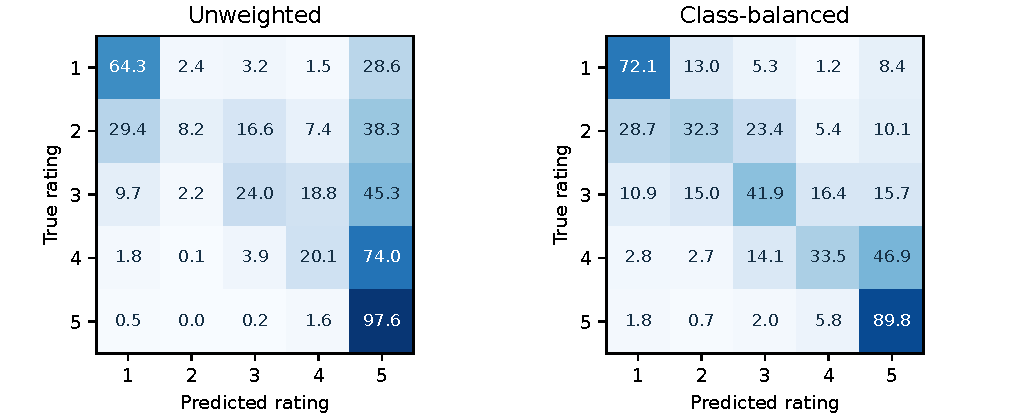
\includegraphics[width=0.91\textwidth]{figures/confusion.pdf}
\caption{Row-normalized validation confusion matrices for the prespecified seed 17. Left: unweighted TF--IDF classifier. Right: class-balanced TF--IDF classifier. Each row corresponds to a true star rating and sums to 100\% before rounding. These are illustrative runs; the main table averages three seeds.}
\label{fig:confusion}
\end{figure*}

\subsection{Error Analysis and Limits of the Evidence}
Figure~\ref{fig:confusion} separates improvement on common labels from recognition of intermediate ratings. For seed 17, two-star recall increases from 8.24\% to 32.33\%, while its precision decreases from 52.08\% to 35.35\%. Five-star recall decreases from 97.61\% to 89.82\%, but five-star precision increases from 76.97\% to 86.20\%. Class balancing therefore shifts the decision boundary toward less frequent ratings rather than improving every precision and recall simultaneously. 

Middle ratings can reflect mixed sentiment and subjective boundaries. A confusion matrix can identify where mistakes concentrate, but does not by itself establish their linguistic cause. Manual inspection will therefore categorize errors involving negation, mixed aspects, short reviews, and long reviews, using a fixed validation sampling rule.

Several limitations remain. First, these are validation results from lexical baselines, not final neural or test results. Second, removing contradictory texts makes the retained task less ambiguous and limits comparability with studies using the raw corpus. Third, exact normalization does not resolve near duplication. Fourth, automated language identification has not been applied; the current corpus is not claimed to be verified English-only data. The English pretrained encoders require a language audit before their input set is frozen. If that audit changes eligibility, a versioned split manifest and rerun baselines will be required, with the original test results still unexamined. Finally, product-disjoint evaluation does not establish user-disjoint, chronological, or cross-domain generalization.

\subsection{Reproducibility Artifacts}
The accompanying folder contains the downloaded archive, its SHA-256 digest, the retained-row split manifest, experiment configuration, per-seed validation predictions, confusion matrices, classwise metrics, and scripts that regenerate the tables and figures. The manifest records original row index, product ID, normalized-text hash, rating, partition, and word count. All report numbers are generated from saved JSON/CSV outputs. The LaTeX source uses the IEEEtran conference class and an IEEE bibliography style. A separate Turkish README explains how to rebuild the report and rerun the experiments.

\section{Next Steps and Completion Plan}
The next stage is to audit language eligibility, near duplicates, GloVe coverage, and tokenizer-specific truncation. These checks will determine whether the present corpus definition can be frozen for the neural study. Next, we will implement TextCNN and DistilBERT training, verify loss gradients and numerical stability, and run a small training-only memory and optimization pilot. After fixing per-architecture budgets, the six validation configurations per loss will be evaluated, followed by three-seed runs of each selected setting.

Only after configuration selection and checkpoint rules are fixed will the reserved test partition be evaluated. The final comparison will include paired differences from CE, the three proposal thresholds, classwise errors, product-level uncertainty estimates, and training time. We will preserve negative or mixed findings rather than select only a favorable metric. Optional All Beauty or another category evaluation is lower priority than completing the six main settings and their replication.

\begin{table}[t]
\caption{Ordered milestones and proposed responsibilities. These are future deliverables, not completed activities or calendar promises.}
\label{tab:next}\centering\footnotesize
\begin{tabularx}{\columnwidth}{@{}P{0.07\columnwidth}Y P{0.23\columnwidth}@{}}
\toprule Step & Deliverable and exit condition & Lead\\\midrule
1 & Language, duplicate, and tokenization audit; freeze data version & Efe Han Kele\c{s}\\
2 & Both neural models and stable losses; pilot logs recorded & Mehmet Ege A\c{s}an\\
3 & Matched validation searches and all three-seed runs & Mehmet Ege A\c{s}an\\
4 & Reserved-test metrics, uncertainty, and error analysis & Faris Aleem Ahmad\\
5 & Final tables, limitations, and checked IEEE PDF & All members\\
\bottomrule
\end{tabularx}
\end{table}

The responsibilities in Table~\ref{tab:next} follow the proposal and can be shared when needed. The main priority is completing the within-architecture loss comparison. Domain transfer and alternative ordinal heads will be attempted only if they do not delay that work. The group will reserve time before the course deadline for checking the final PDF, validating the reported numbers, and preparing a single group submission.

\section{Conclusion}
The project now has a justified experimental design, a reviewed theoretical basis, and a reproducible empirical starting point. The full Fine Foods audit revealed substantial duplication and produced 393,001 retained reviews with product-disjoint partitions. Six linear training runs demonstrated that review text provides useful predictive information beyond the five-star majority baseline and that class balancing improves aggregate performance while changing classwise precision and recall. These findings make a joint nominal/ordinal assessment necessary. TextCNN, DistilBERT, and CE/OLL/MLL comparative training have not yet been performed, so the ordinal-learning hypothesis remains open. Completing that controlled experiment and evaluating it once on the reserved test set are the next central deliverables.

\bibliographystyle{IEEEtran}
\bibliography{references}
\end{document}
